\begin{titlepage}
	\begin{tikzpicture}[remember picture, overlay]
		% Gambar latar belakang atau logo
		\node[anchor=north west, inner sep=0pt] at ([xshift=.18\textwidth, yshift=-.1\textwidth] current page.north west){
			
\includegraphics[width=.3\paperwidth]{../figures/logo_universitas.png} 
		};
	
		\node[anchor=north west, inner sep=0pt, opacity=.12] at (current page.north west){
			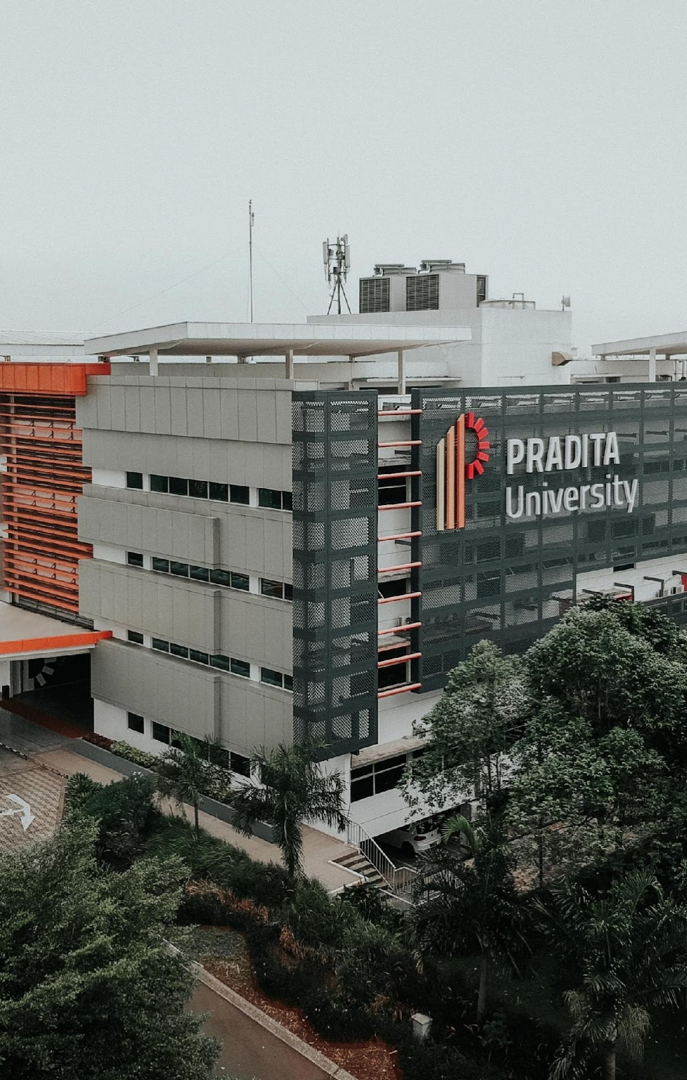
\includegraphics[width=\paperwidth]{../figures/building.png}
		};
		
		% Judul Tengah
		\node[anchor=center] at ([yshift=.1\textheight]current page.center) {
			\begin{minipage}{\textwidth}
				
				{\HUGE \textcolor{praditagreen}{
				\textbf{Rekayasa\vspace{10pt}\\
						Perangkat Lunak\vspace{10pt}\\
						Berbasis Model\vspace{10pt}\\
						untuk DevOps
				}}}\\[0.03\textheight] % Title
				{\LARGE Dari Sistem yang Berjalan sampai Generasi Artefak}\\[.05\textheight] % Subtitle
%				{\Huge \textcolor{praditagreen}{\textbf{Penggunaan Large-language Model}}}\\[.08\textheight] % Subtitle
				{\LARGE \textbf{Alfa Yohannis}}\\[0.05\textheight] % Authors
			\end{minipage}
		};
		
		% Teks bawah dengan latar oranye penuh dan teks putih
		\node[anchor=south west] at (
		current page.south west) {
			\begin{tikzpicture}[remember picture, overlay]
				\node[anchor=south west, fill=praditagreen, text=white, minimum width=\paperwidth, minimum height=.14\textheight, align=center, font=\Huge\bfseries] at (-.15,-.15) {
					Department of Information Technology\\
					Pradita University
				};
			\end{tikzpicture}
		};
	\end{tikzpicture}
\end{titlepage}